%==============================================================================
% Sjabloon poster bachproef
%==============================================================================
% Gebaseerd op document class `a0poster' door Gerlinde Kettl en Matthias Weiser
% Aangepast voor gebruik aan HOGENT door Jens Buysse en Bert Van Vreckem

\documentclass[a0,portrait]{hogent-poster}

% Info over de opleiding
\course{Bachelorproef}
\studyprogramme{toegepaste informatica}
\academicyear{2024-2025}
\institution{Hogeschool Gent, Valentin Vaerwyckweg 1, 9000 Gent}

% Info over de bachelorproef
\title{Geautomatiseerde Analyse van Waargenomen Objecten en Kijkduur\\ met behulp van Hoofd Gemonteerde\\ Eyetracking in Zorgsimulaties.}
\author{Ilian Bronchart}
\email{ilian.bronchart@student.hogent.be}
\supervisor{Bert Van Vreckem}
\cosupervisor{Jorrit Campens}

\specialisation{AI \& Data Engineer}
\keywords{Objectherkenning, Eyetracking, Zorgsimulaties, Verpleegkunde}
\projectrepo{https://github.com/ilianbronchart/bachelorproef}

\begin{document}

\maketitle

\begin{multicols}{2} % This is how many columns your poster will be broken into, a portrait poster is generally split into 2 columns

\section{Introductie}
Observatievaardigheden zijn essentieel in de zorg. 
De huidige, vaak subjectieve, evaluatiemethoden in zorgsimulaties schieten tekort. 
Studenten in de ouderenzorg hebben soms moeite met het observeren van sociale context (fotokader, hobby voorwerpen), 
of zij missen, in de omgang met kleuters, het gevaar van rondslingerende voorwerpen zoals een schaar. 
Vooral voor het accuraat waarnemen van dergelijke objecten levert eyetracking objectieve blikdata. 
Geschikte software ontbreekt echter om automatisch te analyseren \textit{welke objecten} studenten zien en \textit{voor hoe lang}.

Deze bachelorproef richt zich op de hoofdonderzoeksvraag, namelijk:\\ \textbf{Hoe kunnen computervisiemodellen geïntegreerd worden met eyetrackingdata van Tobii Glasses om observatieprestaties van studenten in het 360° Zorglab automatisch te analyseren?} \\
De volgende deelvragen werden hierbij beantwoord:
\begin{itemize}
  \item Welke barrières (cognitief, technisch, didactisch) beperken huidige handmatige observatiemethoden?
  \item Aan welke kenmerken moet een geautomatiseerde analysemethode voldoen om deze beperkingen te verhelpen?
  \item In welke mate kan de ontwikkelde software:
    \begin{enumerate}
      \item correct bepalen welke kritische objecten studenten waarnamen?
      \item nauwkeurig meten hoe lang studenten naar deze objecten keken?
    \end{enumerate}
\end{itemize}
Een proof-of-concept (PoC) software werd ontwikkeld, met als doel een objectieve, datagestuurde basis te leggen om de feedback aan studenten te verbeteren.

\section{Methodologie}
De onderzoeksmethodologie omvatte de volgende fasen (zie figuur hieronder):
\begin{itemize}
  \item \textbf{Literatuurstudie \& Oplossingsverkenning:} Grondig onderzoek naar eyetracking, Computer Vision (CV) modellen (YOLO, SAM, DINOv2) en selectie van de meest belovende analysepijplijnstrategie.
  \item \textbf{Huisgemaakte Eyetrackingdata:} Initiële dataverzameling met de Tobii-bril om de werking te begrijpen en de PoC-ontwikkeling te informeren.
  \item \textbf{Ontwikkeling PoC Software:} Implementatie van een webapplicatie (Python, FastAPI, HTMX) met o.a. een semi-automatische labeling tool (o.b.v. SAM2) voor objectsegmentatie en -tracking.
  \item \textbf{Experimenteel Onderzoek:} Verzamelen van een onbevooroordeelde dataset aan eyetracking-opnames in het Zorglab met zorgrelevante objecten aan de hand van een observatietaak, door studenten uitgevoerd. Output: Twee kalibratieopnames (door onderzoeker) en evaluatieopnames (met studenten). De eerste kalibratieopname toonde objecten met dezelfde achtergrond als de evaluatieopnames (enkel deze werd gebruikt); de tweede met een afwijkende achtergrond.  
  \item \textbf{Creatie Grondwaarheidsdataset:} Labelen van de evaluatieopnames m.b.v. de PoC-tool en filteren op basis van blikdata. Output: Een per-frame gelabelde dataset van daadwerkelijk bekeken objecten.
  \item \textbf{Implementatie \& Evaluatie Analysemethoden:} Toepassen van de gekozen pijplijn (FastSAM-tracking, blikgestuurde filtering, YOLOv11-objectdetectie) op de evaluatieopnames. Output: Prestatiescores (precisie, recall, F1) t.o.v. de grondwaarheid.
\end{itemize}
\vspace{5pt}
\begin{center}
  \captionsetup{type=figure}
  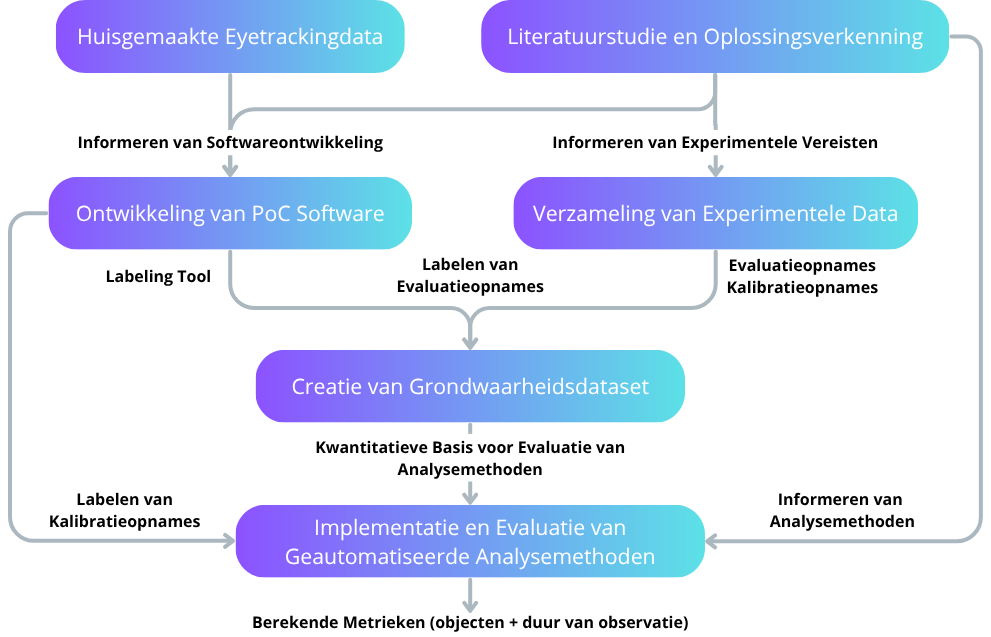
\includegraphics[width=1.0\linewidth]{methodologie.png}
\end{center}

\section{Labeling Tool}
Een kerncomponent van de ontwikkelde PoC-applicatie is de semi-automatische labeling tool (zie figuur hieronder). 
Deze stelt gebruikers in staat om met slechts enkele klikken een object in een videoframe aan te duiden, 
waarna het SAM2-model dit object efficiënt segmenteert en automatisch volgt (trackt) doorheen de opname. 
De output was van belang voor:
\begin{itemize}
  \item Het creëren van de grondwaarheidsdataset op basis van \textit{evaluatieopnames} voor het evalueren van de analysepijplijn.
  \item Het genereren van trainingsdata op basis van \textit{kalibratieopnames} voor de objectdetectiemodellen binnen die pijplijn.
\end{itemize}

\begin{center}
  \captionsetup{type=figure}
  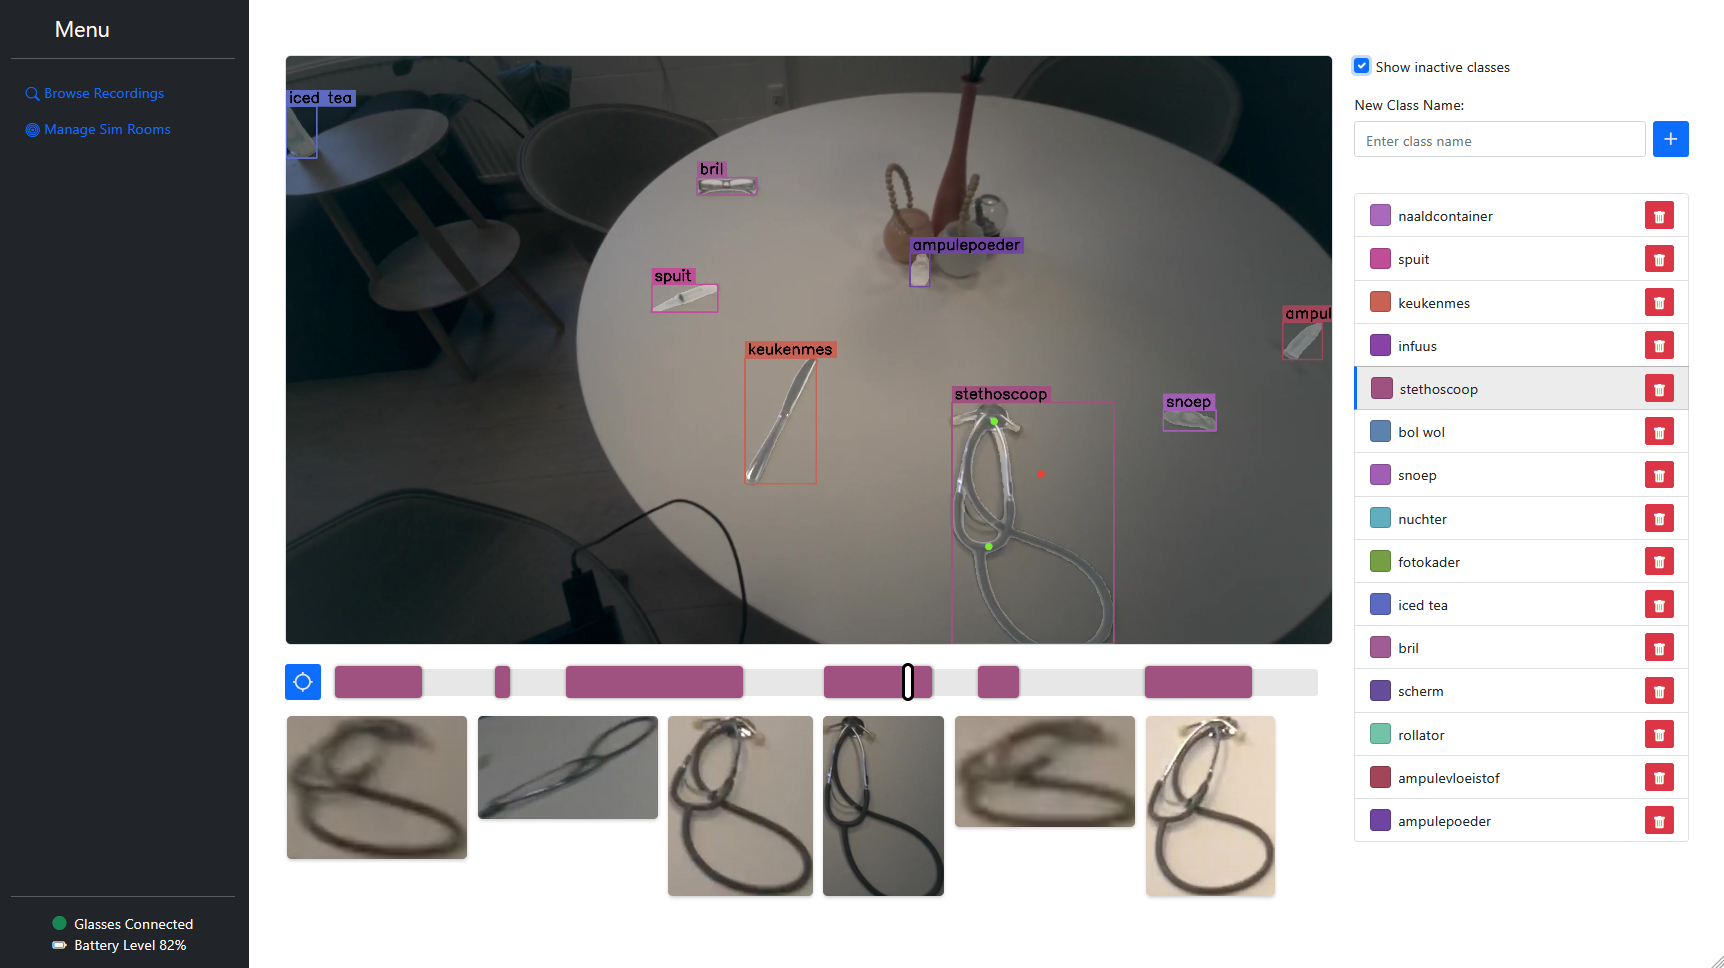
\includegraphics[width=1.0\linewidth]{labeler.png}
\end{center}

\section{Analysepijplijn}
Om de eyetrackingdata automatisch te analyseren, werd een pijplijn geïmplementeerd en geëvalueerd, die de volgende stappen omvat:
\begin{enumerate}
    \item \textbf{Segmentatie \& Tracking:} FastSAM segmenteert en volgt alle potentiële objecten in de videoframes van de evaluatieopnames.
    \item \textbf{Filtering:} De resulterende segmenten worden gefilterd op objectgrootte en daadwerkelijke observatie (overlap met blikpunt student).
    \item \textbf{Classificatie:} De overgebleven, bekeken segmenten worden\\ geclassificeerd m.b.v. een getraind YOLOv11-objectdetectiemodel.
\end{enumerate}
De prestaties werden geëvalueerd t.o.v. de grondwaarheidsdataset. De combinatie van FastSAM-tracking met een YOLOv11-objectdetector (getraind op 1000 voorbeelden per klasse) leverde de beste resultaten op:
\begin{center}
  \captionsetup{type=figure}
  
\includegraphics[width=1.0\linewidth]{results.png}
\end{center}

\section{Conclusies}
Deze bachelorproef demonstreert de haalbaarheid van geautomatiseerde analyse van observatievaardigheden in zorgsimulaties door computervisie en eyetracking te integreren. 
De ontwikkelde PoC-software biedt een basis voor verder onderzoek door middel van de labeling tool.

De geëvalueerde analysepijplijn behaalde veelbelovende resultaten met een hoge precisie (0.94) en een F1-score van 0.80. 
Analyse toonde aan dat veel `vals-positieven' in werkelijkheid correct gedetecteerde objecten waren die door een mismatch met FastSAM-segmentaties niet in de grondwaarheid voorkwamen.
Dit maakt de precisie in de realiteit nog hoger.
De lagere recall (0.70) werd voornamelijk veroorzaakt door uitdagingen bij het consistent detecteren van kleine, transparante of laaggecontrasteerde objecten.
Het variëren van het aantal trainingsvoorbeelden per klasse had geen enkele invloed op de prestaties. 
Dit suggereert dat de beperkende factor niet ligt bij de objectdetectiestap, maar eerder bij de segmentatie- en trackingstap.

Ondanks deze beperkingen zet dit werk een belangrijke stap richting een objectieve, datagestuurde basis om de feedback aan studenten in de toekomst te verbeteren.

\section{Toekomstig onderzoek}
\begin{itemize}
  \item \textbf{Optimalisatie:} Verbeteren van recall door FastSAM-optimalisatie, robuustere tracking/segmentatiemethoden, onderzoek naar end-to-end modellen.
  \item \textbf{Validatie \& Generalisatie:} Testen in meer realistische scenario's, met een grotere variëteit aan objecten en achtergronden.
  \item \textbf{Software-uitbreiding:} Integratie van een analyse- en visualisatiemodule in de PoC, en toevoegen van andere computervisie-taken (bv. gezichtsherkenning).
  \item \textbf{Hardware Overwegingen:} Investering in een GPU voor het Zorglab en evaluatie van eyetrackers met hogere resolutie en/of betere camera's.
  \item \textbf{Methodologie Grondwaarheid:} Verfijnen van de definitie van `bekeken' objecten om nuances beter te vatten.
\end{itemize}

\end{multicols}
\end{document}